\chapter{Basics of Cavitation}
\label{chap:chapter1}
\section{Definition of cavitation}
Cavitation occurs when the pressure is lower than the vapor pressure in a liquid medium at a given temperature. The formation of vapor bubbles is considered to be void space, 
a cavity, and a region of the fluid in which vapor exists are called cavities. These vapor cavities inside a homogenous liquid (in the absence of bubbles in the fluid stream) can occur in many different conditions based on
the characteristics of liquids that vary depending on the flow configuration and the physical properties of the liquid.\\

According to Fran and Michel\cite{FundamentalsofCavitation.2004}  "Cavitation can be defined as the breakdown of a liquid medium under very low pressure".
This makes cavitation relevant to the field of continuum mechanics and it applies to cases in which the liquid  is either statics or motion.
 \\
\section{Tension in Liquid}
The tension of the liquid means, the liquid at 
 constant temperature could be subject to a decreasing pressure p, which falls below the saturation vapor pressure. The value of $P_v$-P is called tension,$\Delta$P and the magnitude at which the rupture
 occurs is the tensile strength of the liquid,$\Delta P_C$. The process of rupture in a liquid at a roughly constant temperature is often called cavitation.
 The maximum negative pressure about which water gets ruptured (in the absence of dissolved gas) ranges between $-3\cdot 10^9$ to $ -3\cdot 10^{10} $ kg/m$s^2$.
\section{Concept of Vapor Pressure} 
 The concept of vapor pressure from the classical thermodynamic viewpoint in the phase diagram of water is shown in (Figure 1.1). It says that the curve from the triple point Tr to the critical point C separates the liquid 
 and vapor domains. The condition of evaporation or condensation of the fluid at a pressure Pv is known as vapor pressure and this is the function of temperature T.
 Cavitation in the liquid occurs by lowering the pressure at a constant temperature as often happens in real fluids. Thus cavitation appears similar to boiling, with exception of the fact that the driving mechanism is not the temperature but 
 pressure change. So the path in the phase diagram is said to be isothermal.\\
 \begin{figure}[H]
    \centering
    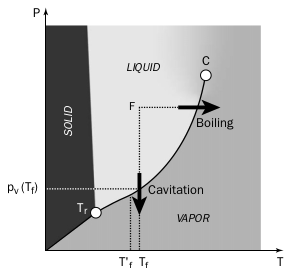
\includegraphics[scale=0.4]{phase diagram.png}
    \caption{phase diagram}
    \label{fig:fig1}
\end{figure}

 
  Several steps can be distinguished during the first instants of cavitation:
  \begin{itemize}
  \item breakdown or void creation,
  \item filling of this void with vapor,
  \item eventual saturation with vapor.
  \end {itemize}
  In reality, the phases are simultaneous with the second step so instantaneous saturation of the void with vapor can be justifiably assumed. It should be kept in mind that from the phase diagram the curve Pv(T)
  is not an absolute boundary between liquid and vapor states. Deviation from this curve can also make the water not change its phase, even if a drop in pressure well below the vapor pressure occurs. This was explained by Andrews-isotherms (Figure 1.2) in the p-v diagram,
the curves can be approximated in the liquid and vapor domains by the van der Waals equation of state. The transformation from liquid to vapor along the path AM can be avoided, because the liquid is in
metastable equilibrium and even can withstand negative absolute pressure i.e, tension, without any phase change special care must be taken for such cases while treating water for the experiment.\\
  
 
\begin{figure}[H]
    \centering
    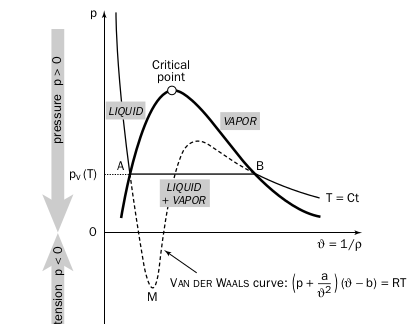
\includegraphics[scale=0.4]{ANDREW ISOTHERM.png}
    \caption{Andrews-isotherms}
    \label{fig:fig2}
\end{figure}
In conclusion, even if the local absolute pressure is equal to or less than the vapor pressure at the given global system temperature does not ensure that the cavitation occurs. This is due to the metastable equilibrium of fluid. This difference between the
vapor pressure and absolute local pressure at cavitation inception(the first point about which phase changes start to generate vapor bubbles)is called static delay. In some cases, there is also dynamic delay is 
associated with inertial phenomena with the time necessary for vapor cavities to be observable.\\
\section{The Main Forms of Vapor Cavities}
Cavitation patterns of vapor structures can be divided into three forms. These are
\begin{itemize}
\item Transient isolated bubbles: These appear in the region of low pressure well below the vapor pressure as a result of the rapid growth of very small air nuclei present in the liquid. They are carried along the 
stream and modify the flow. As they enter into a region of high pressure they progressively disappear.
\item Attached or Sheet Cavities: Such cavities are often attached to the leading edge of the body.
\item Cavitating Vortices: Cavitation can appear in the low-pressure core of the vortices in the turbulent wake.
\end{itemize}
Some vapor structures with a short lifetime that appear on the surface of the foils or propeller blades do not fall under these three forms; even though they have the form of attached cavities, 
they are transported similarly to traveling bubbles. This type of form was taken place in this model.\\
\section{Cavitation Regimes}
For practical purposes, it is necessary to classify the cavitation region.
\begin{itemize}
\item Cavitation Inception: the limiting regime between the non-cavitating condition and the cavitating flow.
\item Developed Cavitation: the where there is an extent of the cavitation zone or significant fall in the performance of the machines.
\end{itemize}
In this work, we are mainly concerned about the extended region of the cavitation zone where there will be a high influence in unsteady cavitation shedding. The influencing situation that is favorable for the 
cavitation is wall geometry which gives rise to the local increment in the velocity with the drop in local pressure, and shear flows due to large turbulent pressure fluctuations.\\
\section{Introduction to Nucleation}
The existence of a point of weakness in the liquid due to the formation of small gas and vapor inclusions and operate at the starting points of the liquid breakdown. They are known as cavitation nuclei. They are 
in a few micrometers and some hundreds of micrometers. They remain spherical at this scale due to surface tension. There are two types of nucleation  are
\begin{itemize}
\item Homogeneous nucleation: when the pressure is well below the saturation pressure the liquid form temporary, microscopic voids that can constitute the nuclei, necessary for rupture and growth of bubbles.
\item Heterogeneous nucleation:  nucleation might occur at the junction of the liquid and solid boundary or due to the contaminant very small sub-micron sized particles in the liquid or due to the
contaminant gas particles as micro-sized bubbles which could present in the crevices within the solid boundary or within the suspended particles or could freely suspend in the liquid which could cause 
 weakness of the fluid under operation.
 \end{itemize}
 Kinetic theories have also been developed to cover such heterogeneous nucleation and allow us to evaluate whether the chance that this will occur is larger or smaller than the chance of homogeneous nucleation.
 Another effect that has less in contributing nucleation is cosmic radiation i.e. the collision of molecules due to high energy photon cause nucleation, but it has little chance to occur so we neglect these
 effects from this work. In most cases, heterogeneities inside the homogeneous medium are taken into consideration because it is inevitable.\\
 Few things that we need to remember that, completely removing contaminated gas from the water is impossible so this effect must be taken into consideration. So it is completely dependent on the
 experiment data because including this weakness in the numerical simulation is impossible so some external parameters have to be implemented which can provide these effects. This is why the reason we include a non-dimensional parameter called cavitation number and cavitation inception
 in this work.\\
 \section{Homogeneous Nucleation Theory}
 Why this theory is important?
 This theory is the basic understanding of the Rayleigh-Plesset equation which is a basic traveling bubble transport equation that will be explained further.\\
 Consider a spherical microbubble, containing gas and vapor(heterogeneous nuclei over homogeneous nuclei) in equilibrium within the liquid at rest. The liquid can withstand negative pressure which means 
 that it is in a metastable state according to Andrews-isotherm cure(Figure 1.2). The bubble radius R which sufficiently smaller so that the hydrostatic pressure $2\rho gR$ can be neglected in comparison with 
 surface tension 2S/R. This condition requires R to be smaller than the limiting value namely 2.7mm for water. This condition is fulfilled in this case because the microbubble whose diameter is smaller than 0.5mm
 only are considered. The pressure can be uniform in the bulk of the surrounding fluid where there is the bubble and this microbubble is spherical. The spherical shape in the bubble is mainly due to
 the surface tension which states that "intermolecular forces that tend to hold the molecules together and prevent the formation of the large hole".\\
 \begin{figure}[H]
    \centering
    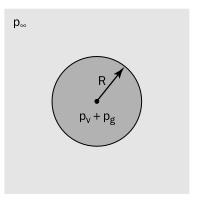
\includegraphics[scale=0.5]{bubble force equilibrium.png}
    \caption{Microbubble in liquid}
    \label{fig:fig3}
\end{figure}
The pressure equilibrium of the interface between the fluid surrounding and bubble surface is given by\\
   \begin{equation}
      P_{\infty} =P_g + P_v -\frac{2S}{R}
      \end{equation}
      ${P_\infty}$ is the surrounding bulk uniform pressure,$P_g$ gas pressure inside the bubble,$P_v$vapor pressure,S surface tension,R radius of the bubble.\\
  It is assumed that pressure change is slow enough to achieve mechanical equilibrium. However, the change in pressure must be rapid enough to ensure the gas diffusion at the interface is negligible.
  In other words, the transformation is assumed to be isothermal and the mass of the gas inside the bubble is constant.\\
  For the initial state,denoted by subscript 0 above equation(1.1)is written by
 \begin{equation}
 P_{{\infty}{0}} =P_{g0}+P_v-\frac{2S}{R_0}
 \end{equation}
 As the gas pressure is inversely proportional to the volume in the isothermal transformation, then the equation(1.1) one can obtain
 \begin{equation}
      P_{\infty} =\frac{P_{g0}}{{[{R_0}/{R}]}^{3}} +P_v -\frac{2S}{R}
      \end{equation}
  Assuming that the critical nucleus is in thermodynamic equilibrium with its surrounding after its creation. The critical radius and critical pressure are given by comparing equation(1.1)$\&$(1.2)by assuming
  virtual transformation from initial radius to critical radius under the isothermal condition with the mass of gas. Two mechanisms take place in equation(1.1), they are
  \begin{itemize}
  \item the internal pressure effect which tend to increase the bubble size,to reach critical size.
  \item the surface tension effect which act in the opposite direction result in extension of minimum given by
  \end{itemize}
  \begin{equation}
  R_C = R_0 \frac {3P_{g0}}{[{\frac{2S}{R_0}}]^{1/2}}
  \end{equation}
  
  \begin{equation}
  P_C = P_v -{\frac{4S}{3R_C}}
  \end{equation}
  The mass of gas is said to be constant and it is directly proportional to the $P_{g0}{{R_0}^3}$.To use the condition of a constant mass of gas either use one of the doublets
   ($R_0 ,P_{\infty}$),($R_0,P_{g0}$) or preferably one of the quantities $R_c or P_c $.The stability of the nucleus is given in (Figure 1.4)in which the mechanical equilibrium of the specific nucleus 
   is stable on the branch of the curve that has a negative slope. The other branch which is on the right side is said to be unstable.\\
   \begin{figure}[H]
    \centering
    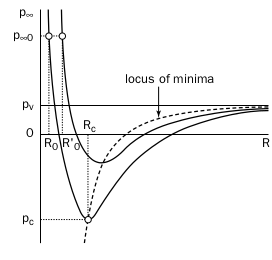
\includegraphics[scale=0.5]{stability curve.png}
    \caption{Equilibrium of a sphere nucleus}
    \label{fig:fig4}
    \end{figure}
    \section{Concept of Cavitation Number}
     The coefficient of pressure $C_{pmin}$ for an ideal fluid is dependent on geometry when the effect of viscosity is included the $C_{pmin}$ is also a function of Reynolds number $R_e$.For this instance we just
    consider only the $C_{pmin}$ as a function of geometry only.
    
    \begin{equation}
    C_{px} =\frac {P_x-P_{\infty}}{{0.5 \rho {U^{2}_{\infty}}}}
    \end{equation}
   The overall pressure decreased or flow velocity increased so that the pressure at some point in the flow approaches the vapor pressure,$P_v$ of the liquid at some reference temperature $T_{\infty}$.In 
   order to relate these natural effects into a parameter, we introduced a new non-dimensional term called Cavitation number $\sigma$. The cavitation number $\sigma$ are related with the $C_{pmin}$ are 
   given below as 
   \begin{equation}
   \sigma =\frac{{P_{\infty}}-{{P_v}(T_{\infty})}}{{0.5 \rho {U^{2}_{\infty}}}}
   \end{equation}
  For sufficiently large value of $\sigma$ ($P_\infty$ sufficiently large compared with $P_v$$(T_\infty)$ or $U_\infty$ sufficiently small), single-phase liquid flow will occur.When $\sigma$ reduced 
  nucleation will first occur at some point for the corresponding value of $\sigma$ called as inception cavitation number ${\sigma}_i$. The minimum pressure point is the point about which nucleation starts 
  observable i.e. vapor bubble, for this instance, neglecting the effect of dynamic delay which deals with inertial phenomena and as per the concern with minimum pressure point in which pressure is less than or equal to the saturated
  vapor pressure. Further reduction $\sigma$ well below ${\sigma}_i$there in an increase in the formation of bubbles. \\
  By the by $C_{pmin}$ as a geometry function the condition of non-cavitation and cavitation are stated below. From the consideration of the minimum pressure point as a first starting point for the nucleation, we 
  relate that point to ${\sigma}_i$ as 
  \begin{equation}
  {{\sigma}_i} =-C_{pmin}
  \end{equation}
  From the Figure(1.5),for $\sigma >$ $-C_{pmin}$ the pressure along the entire trajectory is greater than vapor pressure $P_v$ and still non-cavitating condition is respected.For $\sigma =$ $-C_{pmin}$,the nucleus encounters $P=P_v$only for infinitesimal moment where observable of nucleus is limited
  or might not be observed.For $\sigma <$ $C_{pmin}$,the nucleus experience $P<P_v$for the finite time where it is observable and travel along the streamline.\\
  \begin{figure}[H]
    \centering
    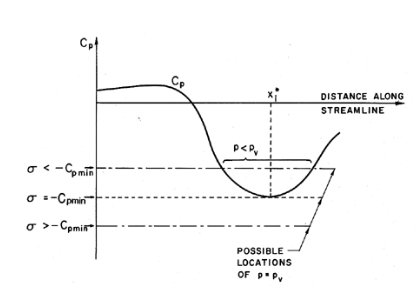
\includegraphics[scale=0.5]{pressure distribution for cp.png}
    \caption{Schematic of pressure distribution on a streamline}
    \label{fig:fig5}
\end{figure}

  In so far as free stream nucleus (heterogeneous nuclei) are concerned two main factors that cause ${\sigma}_i$ be different from $C_{pmin}$.
  The first nucleation may not occur at $P=P_v$.In a degassed liquid, nucleation requires positive tension $\Delta P_c$ and hence nucleation would require the cavitation number ${{\sigma}_i} <$$C_{Pmin}$, namely the equation relating the terms like $C_{pmin}$ and tension of the fluid i.e.
  ${{\sigma}_i}=$${-C_{pmin}}-$$\frac {{\Delta}P_c}{0.5 \rho {{{U}^2}_\infty}}$.In a liquid containing great deal of contaminant gas $\Delta P_c$ could be negative so that ${\sigma}$ would be larger than ${-C_{pmin}}$under the condition $P<{P_v}-$${\Delta}P_c$.This makes the
  ${{\sigma}_i}<$${-C_{pmin}}-$$\frac {{\Delta}P_c}{0.5 \rho {{{U}^2}_\infty}}$.All these conditions should respect the assumption of isothermal. If we include the temperature then ${\sigma}_i$will also
  be the function of Temperature. Finally concluded by, when there is a great deal of contaminant gas the tension of the fluid ${\Delta}P_c$ is negative which means less tension and rupture of fluid will
  occur faster and less in metastable equilibrium. In another sense, positive tension in the case of degassed fluid provides control in cavitation. So not only the geometry but also treating fluid for the experiment 
  is also contributed for the cavitation.
  \section{Viscous effect in cavitation inception}
  Why do we need to get cavitation inception through experiments to strengthen this work?
  The best example, In real fluid, $C_{pmin}$ is not only the function of geometry but also the contribution by the viscosity. To include this effect of viscosity the $C_{pmin}$ would be the function of 
  Reynolds number,$R_e$ so the cavitation inception,${\sigma}_i$ is a dependence of Reynolds number,$R_e$. In most, engineering applications the flow is said to be turbulence so the vortices occur not only 
  because of the inheritance of turbulence but also due to free and forced shedding of vortices. This has major consequences in the cavitation inception ${\sigma}_i$ because the pressure at the center part of the 
  vortices is lower than the mean pressure in the flow so the cavitation first occurs at the core. So ${\sigma}_i$ will changes with $R_e$. This shows how the turbulence effect ${\sigma}_i$. There are a few other effects that 
  make the ${\sigma}_i$ to be more complicated in measurement through experiment.
  \begin{itemize}
  \item Existence of tensile strength can cause a reduction in ${\sigma}_i$.
  \item Residence time effects can cause a reduction in ${\sigma}_i$.
  \item Existence of contaminated gas can cause an increase in ${\sigma}_i$.
  \item Steady viscous effect due to dependence of $C_{pmin}$ on $R_e$ can cause ${\sigma}_i$ to be function of $R_e$.
  \item Turbulence effect can cause an increase in ${\sigma}_i$
  \end{itemize}
  If these effects are not included then ${\sigma}_i$ is only function of $C_{pmin}$.Some of the experiment technique which is used to measure the ${\sigma}_i$ is the device based on acoustic scattering and light
  scattering have been used to measure the number of nuclei present in the liquid. Other instruments known as cavitation susceptibility meters cause a sample of liquid to cavitate and measure the number and size of the 
  resulting microscopic bubbles. The discussion of this technique is out of the scope of this topic.
  \section{Types of Cavitation}
  \subsection{Travelling Bubble Cavitation}
  The bubble began as micron-sized nuclei in the liquid of the oncoming stream and the bubble moved with the flow free stream velocity close to the solid body.Cavitation inception was deemed to occur 
  when the bubble reaches an observable size.
  \begin{figure}[H]
    \centering
    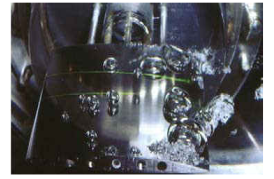
\includegraphics[scale=0.6]{travellingbubble.png}
    \caption{Travelling bubble on the surface of an hydrofoil}
    \label{fig:fig6}
\end{figure}
\subsection{Vortex Cavitation}
  This type of cavitation comes under large-scale cavitation structures. Cavitation inception often occurs at the core of the vortices when the core pressure is well below the mean flow pressure.
For high $R_e$ the vortices in a turbulent mixing layer or wake will also cavitate. This type is often seen in the tip vortices in the ship's propellers or pump impellers.
The three-dimensional shedding of vortices from a finite aspect ratio foil often leads to the formation and propagation 
of a ring vortex with a vapor core. In this work, there is only two-dimensional analysis so three-dimensional shedding is excluded.
\begin{figure}[H]
 \centering
 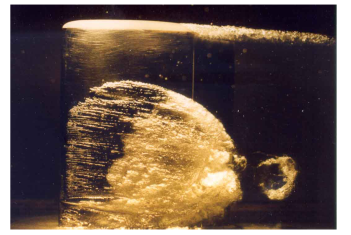
\includegraphics[scale=0.5]{Vortexcavitation.png}
 \caption{ring vortex on the surface of an hydrofoil}
  \label{fig:fig7}
\end{figure}
\subsection{Cloud Cavitation}
This is another class of large-scale cavitation. The periodic formation and collapse of a cloud of cavitation bubbles are observed. This is the area of interest where we simulate to generate cloud shedding.
 \begin{figure}[H]
 \centering
 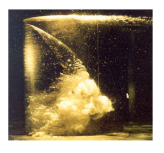
\includegraphics[scale=1]{cloudshedding.png}
 \caption{Cavitating cloud on hydrofoil}
  \label{fig:fig8}
\end{figure} 
\subsection{Shear Cavitation}
The region with high shear vorticity produces.  As a result, a coherent rotational structure is formed and pressure levels drop in the core of the vortices which became the potential site for the cavitation. This 
often happen in the flow separation region which is developed by the hydrofoil at very high $R_e$ and angle of attack.
\begin{figure}[H]
 \centering
 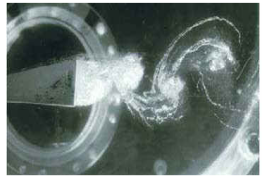
\includegraphics[scale=0.6]{shearcavitation.png}
 \caption{Shear Cavitation}
  \label{fig:fig9}
\end{figure}
\subsection{Attached/Sheet Cavitation}
These types of cavitation are often experienced in hydrofoils. In this work Attached/Sheetcavitation was been simulated through the case setup and this is the area of interest to replicate the unsteady behavior of cloud shedding.\\
\textbf{SuperCavitation}: As the cavitation parameter is decreased a small cavity attached to a hydrofoil will extend to grow longer and longer. It is because a super cavity as soon as it ceases to close the cavitation
wall but inside the liquid downstream of the cavitation. Simultaneously the lift of the foil will decrease and the drag will increases. For lower cavitation number which means low $R_e$ the supercavitation 
would experience in the foil and cavity closure will occur at the rear part. Because of lower in $R_e$ laminar separation boundary layer would experience over the hydrofoil. They showed that a well-developed 
cavity always detached downstream of laminar separation of the boundary layer. The existence of separation, which generates a relatively dead zone near the downstream is the only way for the cavity to get attached to the wall. Because 
of the transition to turbulence, the eddy in the flow tries to fix the layer near to the wall due to momentum transfer from the outside of the boundary layer to the inner layer of the flow stream is to overcome the adverse pressure effect. If there is no separation the cavity 
will be swept away by the flow. The cavity closure will be experienced on the rear part due to the cavity pressure which is lower than the surrounding pressure. The unbalance inertia and pressure force gives a 
curvature oriented toward the cavity.\\
\begin{figure}[H]
 \centering
 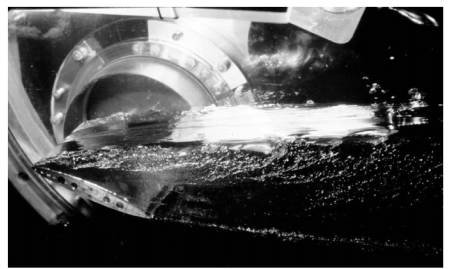
\includegraphics[scale=0.4]{supercavitation.png}
 \caption{Supercavity behind two dimensional hydrofoil}
  \label{fig:fig10}
\end{figure}

\textbf{Partial Cavitation}: This topic is the important one that is completely followed in the entire work and the condition which is represented in this topic is the real condition that was followed in the numerical
 case set up to generate the partial cavity. In partial cavitation, the attached cavity closes on the suction side of the hydrofoil. This type of cavitation has two types,

\textbf{Open attached cavity -partial type}: It is typically frothy in appearance and has periodically varying lengths, which is associated with the shedding of vapor clouds. The re-entrant jet was not observed 
in the cavity closure although recirculation flow associated with the region of separation of flow was detected and there is turbulent reattachment. The reason for the non-observation of the re-entrant jet in an open cavity
because there should be a condition related to the maximum cavity thickness which was not attained in the open cavity because of low cavitation number is associated with the low angle of attack for the case of hydrofoil
which can be seen in the figure.\\
\textbf{Closed attached cavity-partial cavity}: This has a relatively stable cavity length, a clear interface, and a cavity closure that is relatively free from the bubble and completely vapor fill. This 
shows an important aspect of introducing the single-phase flow concept by considering the vapor-filled state because bubble interaction is completely removed from the above statement of the closed partial cavity 
and assuming relative velocity between these two-phase as zero means now the flow completely transfers to a single-phase flow regime. This closed partial cavitation is being adapted in this simulation for 
unsteady cloud shedding and re-entrant jet observation.\\
\begin{figure}[H]
 \centering
 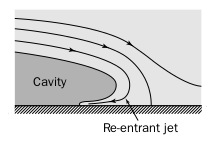
\includegraphics[scale=1]{reentantjet.png}
 \caption{closure region of partial cavity}
  \label{fig:fig11}
\end{figure}
 \textbf{Unsteady Re-entrant jet}: The re-entrant jet which travels from the upstream carrying small quantity of liquid inside the cavity and the outer region reattached by turbulent reattachement.The unsteady 
 re-entrant jet cavity is largely vapor-filled the cavity interface is close near the suction rear side where maximum cavity length is observed
from a thin re-entrant jet flow. This re-entrant jet causes the cavity to periodic break-off and roll-up of a portion of the cavity when they impinge on the cavity interface. If the re-entrant jet moves far upstream to cause a large portion of the cavity to 
break off the process creates large-scale cloud shedding. If they move to a smaller distance upstream before impingement on the cavity surface then the process is called small-scale cloud cavitation.

 From the figure(1.12) we can see that the open cavity at low cavitation and low angle of attack where the re-entrant is not observed or weak in re-entrant flow but there is a turbulent reattachment. At the
same time in the periodic zone regime, we can see cloud shedding at a higher angle of attack and higher cavitation number along with the ratio of cavitation thickness to the chord $e/c$ is minimum and 
the ratio of the length of the cavity to chord $l/c$ is around half the length of the chord act as a maximum $l/c$ i.e. a peculiar instability develops for partial cavities of medium length. On the other hand, it was limited 
by the minimum cavity thickness. Such limits suggest that a minimum value of cavity thickness is required for the periodic regime to develop. This also shows that cavity thickness must 
be larger than the re-entrant jet thickness for this instability to occur along with another condition like the periodic regime is bounded by the maximum value of the cavity length which indicates that instability 
should not occur for very long cavities. This condition also holds for the re-entrant jet which requires a minimum threshold value of the adverse pressure gradient to gain the impulse. Finally concluding this topic by, 
there must be minimum cavity thickness to chord ratio simultaneously maximum length of the cavity to chord ratio is required to obtain partial periodic cavity shedding along with energetic re-entrant jet. These conditions are 
well respected in this work for such kind of observation.\\
\begin{figure}[H]
 \centering
 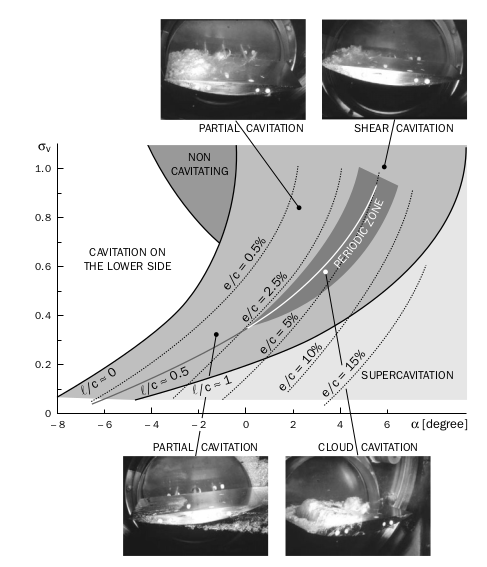
\includegraphics[scale=0.4]{partialcavitation.png}
 \caption{Main cavity patterns at $R_e =$ $2.{10}^6$ ${V_{\infty}} =10{m}/{s}$ on plano-circular hydrofoil.l is the cavity length(maximum in the case of an unsteady cavity )and e the maximum thickness of the cavity.\\}
  \label{fig:fig12}
\end{figure}
\section{Three dimensional effect in hydrofoil}
The transition of sheet cavitation to cloud cavitation can result in a highly unstable flow.To study cavitation-vortex interaction\cite{JI2015}, the vorticity transport equation in a varying  density 
flow is given as 
\begin{equation}
\frac{D\omega}{Dt}=({\omega.\triangledown})\vec{V} -\vec{\omega}(\triangledown.\vec{V}) + \frac{{\triangledown{\rho}_m} {\times\triangledown P}}{{{\rho}^2}_m} +({\nu}_m +{\nu}_t){{\triangledown}^2}\vec{\omega}
\end{equation}
In this equation, the first term on the right-hand side(RHS)is the vortex stretching the term. This term represents the stretching and tilting of a vortex by velocity gradients. The second term on the RHS
is the vortex dilation term due to volumetric expansion/contraction, which describes how the fluid compressibility affects the vorticity. The third term on the RHS is the baroclinic torque which is due to 
misaligned pressure and density gradients. The last term on the RHS indicates the rate at which the vorticity changes due to viscous diffusion of the vorticity. Note that the viscous diffusion term has a much smaller
effect on the vorticity transport than the other three terms in high $R_e$ because away from the wall inertia force is more dominant than viscous force. The numerical and experimental studies show
that there is strong vortex-cavitation interaction in the shedding vapor and the vortex stretching and dilatation is the primary mechanism of transition of cloud from 2D to 3D cloud as the shedding 
vapor cloud collapse downstream the attached cavity shrinks quickly and changes from 3d to 2D. During this process, the attached sheet cavity and the boundary layer became very thin. The strength of the vortex 
stretching term and dilatation term decreases significantly along with the extent of the cavitation region. Even though the magnitude of the baroclinic torque term is smaller if compared with the vortex stretching 
term and dilatation term, the baroclinic torque is very important for the production of vorticity and modifies the vorticity field in the region with high density and pressure gradient i.e. along with liquid-vapor 
interface and near the cavity closure. Even though it is a miscellaneous topic for this work but important to understand the 3D effect in hydrofoil and this effect reflect in the result while comparing numerical
2D with the experimental result.

\section{Main Effect of Cavitation in Hydraulics Performance}
\begin{itemize}
\item drop down the performance of the hydraulics system like reduction in lift and increase in drag of the foil, fall turbomachinery efficiency, reduced capacity to evacuate water in spillways, energy 
dissipation, etc.
\item the appearance of additional forces in the solid structures.
\item production of noise and vibration,
\item wall erosion when the bubble gets extruded between the fluid and solid surface caused the solid surface to erode and this effect  acts like a creep where it reduces the useful lifetime of the machine.
\end{itemize}

\chapter{Theoretical Formulation}
\label{chap:chapter2}
\section{Governing Equation}
The basic governing equations of single-phase flow comprises mass, momentum conservation are given below. The energy equation is neglected because the change in flow properties is taking place in the isothermal condition.
From the single-phase flow conservation equation, we will extract the equations for multiphase flow based on the assumption stated in\cite{CavitationandBubbleDynamics.1995,Hidalgo2014}.\\
\subsection{Homogeneous bubbly flows}
From homogeneous nucleation, theory \cite{FundamentalsofCavitation.2004}the microbubbles whose diameter is smaller than 0.5mm only are considered so that hydrostatic pressure can be neglected in comparison 
with surface tension. When the concentration of the bubbles in the flow exceeds these values the bubble will have a significant effect on the fluid dynamics of the suspending liquid.
Then the analyses of the multiphase mixture will become too complex. In the large context of practical multiphase flows, one can find a wide range of homogeneities i.e. consisting of one phase that is very finely 
dispersed with the other phase of two-phase flow with a separate stream. The two asymptotic states are commonly referred to homogeneous and separated flows. They are often called homogenous mixture flows in 
the computational domain. The important aspect of this kind of flow is defining the relative motion between the two phases because two streams will move in different velocities and such 
relative motion between two phases is an implicit part of the study of separated flow. But based on the assumption, such as two-phase flows are sufficiently well mixed and the disperse 
particle size sufficiently small in order to eliminate any significant relative motion. Thus the term homogeneous flow some times used to denote a flow with the relative motion to be zero. 
Many bubbly flows will come close to this approximation. In the absence of relative motion the governing mass and momentum conservation equations reduce to a form similar to those for single phase flow.
It is possible to establish barotropic relation which controls the condensation$\&$vaporization and this allows one to anticipate that entire spectrum of phenomena observed in single-phase flow dynamics.
\subsection{Governing equations}
The dynamic model of cavitation is established by using mixture continuity and momentum equations of RANS turbulence model are stated below\cite{Zhao2021}.
\begin{equation}
\frac{\partial{{\rho}_m}}{\partial t} + \frac{\partial{{{\rho}_m} u_j}}{\partial{x_j}} = 0
\end{equation}
\begin{equation}
\frac{\partial{{\rho}_m}}{\partial t} + \frac{\partial{{{\rho}_m} u_j}}{\partial{x_j}} =\frac{\partial}{\partial{x_j}}\Bigg[{\mu}_m\Bigg(\frac{\partial{u_i}}{\partial{x_j}}+\frac{\partial{u_j}}{\partial{x_i}}\Bigg)\Bigg]
-\frac{\partial}{\partial{x_i}} \Bigg({P}+{\frac{2}{3}}{\mu}_m \frac{\partial{u_k}}{\partial{x_k}}\Bigg) + {{\rho}_m}g_i +\frac{\partial{R_{ij}}}{\partial{x_j}}
\end{equation}

\begin{equation}
R_{ij} = {- \rho \overline{{{u_i}^\prime}{{u_j}^\prime}}} = - \frac{2}{3}\Bigg({\rho}k +{{\mu}_t}\frac{\partial{u_l}}{\partial{x_l}}\Bigg)\delta{ij} + {{\mu}_t}\Bigg({{\frac{\partial{u_i}}{\partial{x_j}}}
+\frac{\partial{u_j}}{\partial{x_i}}}\Bigg) + {\tilde{R_{ij}}}
\end{equation}
The vapour fraction $\alpha$ is used to find density $\rho$ and dynamic viscosity $\mu$ as shown in eqaution below.
\begin{equation}
\alpha =\frac {\forall{V}}{\forall}
\end{equation}
The mixture density and the viscosity are defined as follows.
\begin{equation}
{{\rho}_m} = {{\rho}_l}{{\alpha}_l} + {{\rho}_v}(1-{{\alpha}_l})
\end{equation}
\begin{equation}
{{\mu}_m} = {{\mu}_l}{{\alpha}_l} +{{\mu}_v}(1-{{\alpha}_l})
\end{equation}
The volume fraction transport equation is given by.
\begin{equation}
\frac{\partial{\alpha}_l}{\partial t}+\frac{\partial}{\partial{x_j}} ({{\alpha}_l}{u_j}) = \frac{\dot{m}}{{\rho}_l}
\end{equation}
\begin{equation}
\dot{m}={{\alpha}_l}\dot{m}^{-} + (1-{{\alpha}_l})\dot{m}^{+}
\end{equation}
\begin{equation}
\frac{\partial{{u_j}}}{\partial{x_j}}=\dot{m}\Bigg(\frac{1}{{\rho}_l}-\frac{1}{{\rho}_v}\Bigg)
\end{equation}
In the above equations, ${\rho}_l$ and ${\rho}_v$ are the liquid and vapor density, respectively; ${\alpha}_l$ and ${\alpha}_v$ are the liquid fraction and the vapor fraction, respectively; ${\mu}_m$ is the mixture laminar viscosity and
${\mu}_t$ is the turbulent viscosity; and $\dot{m}^+$ and $\dot{m}^-$ represent the condensation and evaporation rates, respectively.

\section{Basic bubble dynamic equation}
In this simple model\cite{FundamentalsofCavitation.2004}, we consider the dynamic evolution of the spherical bubble with the fixed center, which undergoes uniform pressure variation at infinity. This simple
model demonstrates many practical cases such as bubble collapse, bubble formation from the nucleus, bubble oscillation, etc. Even this model is suitable for more complicated situations, involving the motion of the bubble
center, which can be approximated by this model. The liquid motion induced by a spherical cavity in an infinite medium under the uniform pressure at infinity seems to have been first considered by Besant in 1859.
It was solved for inviscid liquid by Rayleigh in 1917, to explain the phenomenon of cavitation erosion. In 1948, Cole use the model of a spherical bubble containing a non-condensable gas. Plesset in 1954, 
consider the general case of bubble evolution for a viscous and non-compressible flow.
\subsection{Assumptions}
\begin{itemize}
\item the liquid is incompressible and either Newtonian or inviscid;
\item gravity is neglected;
\item mass of the air inside the bubble is constant, its inertia is neglected. The transformation from one radius to another by the bubble take place in isothermal condition;
\item the bubble is saturated with vapor when the local pressure of the liquid is well below the vapor pressure.
\end{itemize}
\begin{figure}[H]
 \centering
 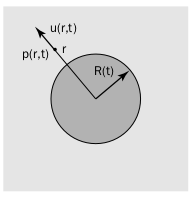
\includegraphics[scale=0.7]{Rayleighplesset.png}
 \caption{Rayleigh Plesset:Evolution of spherical bubble}
  \label{fig:fig13}
\end{figure}
The functions to be determined, in the liquid domain r $\ge$ R(t), are the velocity u(r,t) and the pressure p(r,t) induced by the evolution of bubble as shown in (fig2.1).
\subsection{Boundary and intial condition}
In this derivation, we disregard the mass transfer through the interface, so u(R,t) represents the liquid velocity at the interface as the interface velocity $/dot R=$$[dR]/[dt]$.
For a viscous fluid of kinematic viscosity m, the normal stress at the surface is:
\begin{equation}
{t_{rr}}(R,t)=-P(R,t)+2{\mu}{\frac{\partial{u}}{\partial{r}}}\Bigg{\vert}_{r=R}
\end{equation}
The balance normal force is given by:
\begin{equation}
-{t_{rr}}(R,t)=P_{v}+{P_{g}}(t)-{\frac{2S}{R}}
\end{equation}
where $P_g$ stands for the partial pressure of the gas inside the bubble. With adiabatic gas transformation, the instantaneous gas pressure is related to the initial gas pressure 
$P_{g0}$ using the following expression:
\begin{equation}
{P_{g}}(t)=P_{g0}\Bigg[\frac{R_0}{R(t)}\Bigg]^{3\gamma}
\end{equation}
where $\gamma$ is the ratio of heat gas capacities $C_{pg}$ and $C_{vg}$.
Thus, the pressure on the cavity interface is given by:
\begin{equation}
P(R,t)=P_{v}+P_{g0}\Bigg[{\frac{R_0}{R(t)}}\Bigg]^{3\gamma}-{\frac{2R}{R}}+2\mu{\frac{\partial{u}}{\partial{r}}}\Bigg{\vert}_{r=R}
\end{equation}
Consider the liquid far from the bubble is assumed to be rest so that u($\infty$, t)$\rightarrow$0 and the pressure P($\infty$, t) also denoted $P_{\infty}$(t) is assumed given.
For the initial condition denoted by the subscript 0, the bubble is assumed to be in thermodynamic equilibrium, i.e., $\dot{R}$(0), so the equation(1.2) is satisfied.
\begin{equation}
P_{{\infty}{0}} =P_{g0}+P_v-\frac{2S}{R_0}
\end{equation}
\subsection{Rayleigh-Plesset eqaution}
Based on spherical symmetry, the flow is irrotational and is of the source type (or sink type). The mass consevation of incompressible fluid is given by $\triangledown.{\vec{V}}=0$ that gives:
\begin{equation}
u(r,t)=\dot{R}\frac{{R}^2}{{r}^2}
\end{equation}
The viscous term of the Navier-Stokes equation is zero in this specific case. Thus for both a viscous and non-viscous fluid, the momentum equation is:
\begin{equation}
{\frac{\partial u}{\partial t}}+u{\frac{\partial u}{\partial r}}=-{\frac{1}{\rho}}{\frac{\partial p}{\partial r}}
\end{equation}
By taking equation(2.15) in to account:
\begin{equation}
{\ddot{R}}{\frac{{R}^2}{r^2}}+2{{\dot{R}}^2}\Bigg[{\frac{R}{r^2}}-{\frac{R^4}{r^5}}\Bigg]=-{\frac{1}{\rho}}{\frac{\partial{p}}{\partial{r}}}
\end{equation}
Integrating with respective to r and considering the condition at infinity, one can obtains:
\begin{equation}
{\frac{P(r,t)-{P_{\infty}}(t)}{\rho}}={\ddot{R}}{\frac{{R}^2}{r^2}}+2{\dot{R^2}}{\Bigg[{\frac{R}{r}}-{\frac{R^4}{4r^4}}\Bigg]}
\end{equation}
This equation is similar to Bernoulli's equation for a variable unsteady flow of inviscid liquid. On the other hand when substituting r=R, equation(2.18) gives:
\begin{equation}
{\frac{P(r,t)-{P_{\infty}}(t)}{\rho}}=R{\ddot{R}}+{\frac{3}{2}}{\dot{R^2}}
\end{equation}
Finally, from the equation(2.13) for the pressure at the interface, and noting that:
\begin{equation}
{{\frac{\partial u}{\partial r}}\Bigg{\vert}_{r=R}}=-{\frac{2\dot R}{R}}
\end{equation}
equation(2.19) becomes:
\begin{equation}
 {\rho \Bigg[{R{\ddot{R}}+{\frac{3}{2}}{\dot{R^2}}}\Bigg]}={P_v}-{{P_{\infty}}(t)}+{P_{g0}}{\Bigg({\frac{R_0}{R}\Bigg)^{3\gamma}}}-{\frac{2S}{R}}-4\mu{\frac{\dot R}{R}}
\end{equation}
This equation is called the Rayleigh-Plesset equation, which permits us to determine the temporal evolution of the radius R and simultaneously the pressure field in the liquid when the law $P_{\infty}$
is given. For inviscid liquid, the last term on the right-hand side vanishes. The corresponding equation is known as the Rayleigh equation.
Both the Rayleigh-Plesset equation and Rayleigh equation are differential and enormously non-linear, because of the inertial terms. With the use of the Rayleigh equation, we can solve the problem of bubble collapse and bubble explosion.
In most instances, the inertial forces are dominant and viscosity does no longer plays a huge role. The position of surface tension is often a secondary case of bubble collapse.
\subsection{Schnerr-Sauer mass transfer model}
According to the detailed literature review, the cavitation model used in this study was developed by Schneer and Sauser. The Schneer and Sauser mass transfer cavitation model are derived from a simplified 
Rayleigh-Plesset equation which neglects the second-order derivative of the bubble radius. In reference\cite{Zhao2021, Hidalgo2014}, the vapor fraction was related to the average radius of the gas nucleus and number density.
The condensation and evaporation rates are as follows:
\begin{equation}
{{\alpha}_v}=\frac{{{n}_0}{\frac{4}{3}}\pi{{R}^3}}{\Bigg({n_0}{\frac{4}{3}}\pi{R^3}+1 \Bigg)}
\end{equation}
\begin{equation}
{{\dot m}^+}={C_v}{\frac{{{\rho}_v}{\rho}_l}{\rho}}{{\alpha}_v}{(1-{\alpha}_v)}{\frac{3}{R}}{\sqrt{\frac{2({P_v}-{P})}{3{\rho}_l}}} \\     
({if P<P_v})
\end{equation}
 \begin{equation}
 {{\dot{m}}^-}={C_c}{\frac{{{\rho}_v}{\rho}_l}{\rho}}{{\alpha}_v}{(1-{\alpha}_v)}{\frac{3}{R}}{\sqrt{\frac{2({P}-{P_v})}{3{\rho}_l}}} \\ 
 ({if P>P_v})
 \end{equation}
 where ${m}^+$, ${m}^-$ are the condensation and evaporation rate respectively; $C_v$, $C_c$ are the empirical coefficient for condensation and evaporation, with the value 2, 1 respectively.\\
 The bubble radius can be related to the vapor volume fraction and the bubble number density:
 \begin{equation}
 R=\Bigg({\frac{{{\alpha}_v}}{1-{{\alpha}_v}}}{\frac{3}{4{\pi}{n_0}}}\Bigg)
 \end{equation}
  From the equation of radius the parameter $n_0$ is the number of gas nucleus per unit volume. This is an important parameter and it set as $1.6 \times 10^{13}$ in this thesis.
  
\section{Introduction to Turbulence}
The majority of flows in engineering application encounters turbulence\cite{ANSYS}. Therefore appropriately turbulent model should be essential while dealing with complex turbulence flow problems. 
The main properties of turbulent flows are:
\begin{itemize}
\item High unsteadiness,
\item Three-dimensionality,
\item High diffusivity(turbulent diffusion),
\item Dissipation,
\item Coherent structure,
\item Fluctuations on broad ranges of length and time scales.
\end{itemize}
\subsection{Reynolds-average Navier-Stokes equation}
The Reynolds decomposition of u and p, instantaneous fields are decomposed into a mean and fluctuating part; referred from\cite{pope2000,ANSYS}:
\begin{equation}
{u_i}={\overline{u_i}}+{{u_i}^\prime}
\end{equation}
where ${\overline{u_i}}$, ${{u_i}^\prime}$ are the mean and fluctuating velocity components.
For pressure and other scalar quantities:
\begin{equation}
\phi ={\overline{\phi}}+{{\phi}^\prime}
\end{equation}
where $\phi$ denotes scalar quantities such as pressure, energy, or species concentration.
Substituting expression of this form for the flow variables in to the instantaneous continuity and momentum equations and taking a ensemble average, yields the ensemble-averaged momentum equations. The equation 
written in cartesian tensor form:
\begin{equation}
{{\frac{\partial \rho}{\partial t}}+{\frac{\partial}{\partial {x_i}}}(\rho u_i)}=0
\end{equation}
The ensemble-average momemtum equation is:
\begin{equation}
{{{\frac{\partial}{\partial t}}(\rho u_i)}+{{\frac{\partial}{\partial x_j}}(\rho{u_i}{u_j})}}={-{\frac{\partial P}{\partial x_i}}+{\frac{\partial}{\partial x_j}}{\Bigg[{\mu}\Bigg({{{\frac{\partial u_i}
{\partial x_j}}+{\frac{\partial u_j}{\partial x_i}}-{\frac{2}{3}}{{\delta}_{ij}}{\frac{\partial u_l}{\partial x_l}}}}\Bigg)\Bigg]+{\frac{\partial}{\partial x_j}}\bigg({-}{\rho}{\overline{{{u_i}^\prime}{{u_j}^\prime}}}\bigg)}}
\end{equation}
 Equation(2.28)$\&$ Equation(2.29) are called Reynolds-average Navier-Stokes (RANS) equations. They show resembles with Navier-Stokes equation only the difference is the velocities and other scalars 
quantities are expressed as ensemble-averaged values. An additional term that is present in the RANS equation represents the effect of turbulence. This term $\bigg({-}{\rho}{\overline{{{u_i}^\prime}{{u_j}^\prime}}}\bigg)$
is called Reynolds stresses. This must be modeled to overcome the closure problem(the number of unknown variables is inconsistent with the number of the equations). Different types of turbulence modeling are being used to model this Reynolds stress term which 
is an additional term in the RANS ensemble-momentum equation.

\subsection{k-$\omega$ sst turbulence model}
After a detailed literature review, it is better to use the k $\omega$ sst model for 2D NACA0012 hydrofoil\cite{Zhao2021,ANSYS}. The shear-stress transport(sst) k-$\omega$ model was developed by Menter to effectively 
blend the robust and accurate formulation of the k-$\omega$ model in the near-wall region with freestream independence of the k-$\epsilon$ model in the far-field. The sst k-$\omega$ model is similar to the 
standard k-$\omega$ model but includes the following refinements.
\begin{itemize}
\item The standard k-$\omega$ model and the transformed k-$\epsilon$ model are both multiplied by a blending function and both models are added together. The blending function is designed to be one in the 
near-wall region, which activates the standard k-$\omega$ model and zero away from the surface, which activates the transformed k-$\epsilon$ model.
\item The sst model incorporates a damped cross-diffusion derivative term in the $\omega$ equation.
\item The definition of the turbulent viscosity is modified to account for the transport of the turbulent shear stress.
\item The modeling constants are different.
\end{itemize}
These features make sst k-$\omega$ model more accurate and reliable for a wider class of flows such as adverse pressue gradient flows, airfoil, transonic shock waves, than standard k-$\omega$ model.
\subsection{Transport equation for the sst k-$\omega$ model}
Turbulent kinetic energy equation reads:
\begin{equation}
{{{\frac{\partial {\rho k}}{\partial t}}+{\triangledown \cdot(\rho k \overline{u})}}-{\triangledown \cdot ({{\Gamma}_{k,eff}}\triangledown{k})}}={min(G,{c_1}{{\beta}^*}k\omega)-{{\beta}^*}k\omega}
\end{equation}
\begin{equation}
{{\Gamma}_{k,eff}}={{{\alpha}_k}{{\mu}_t}}+{\mu}
\end{equation}
Specific dissipation rate equation reads as:
\begin{equation}
{{{\frac{\partial}{\partial t}}(\rho \omega)}+{{\triangledown\cdot(\rho \omega \overline{u})}}-{\triangledown({{\Gamma}_{\omega,eff}})}}={{{\gamma}_{min}}\bigg[{S_2},{\frac{c_1}{a_1}}{{\beta}^*}\omega max\bigg
({a_1},{\omega},{b_1}{F_{2}\sqrt{S_2}\bigg)\bigg]}}-{{\beta}{{\omega}^2}+(1-{F_1})CD_{k\omega}}
\end{equation}
\begin{equation}
{{\Gamma}_{\omega,eff}}={{{\alpha}_{\omega}}{{\mu}_t}+{\mu}}
\end{equation}
The eddy viscosity is calculated as:
\begin{equation}
{{\mu}_t}={\frac{{a_1}\rho k}{max\bigg[{a_1}{\omega},{b_1}{F_2}\sqrt{2}\bigg\vert{{\frac{1}{2}\bigg({\triangledown \overline{u}}+{(\triangledown \overline{u})^{T}}\bigg)\bigg\vert }}\bigg]}}
\end{equation}
and the production of turbulent kinetic energy reads:
\begin{equation}
{G}={{\mu}_t}{S_2}
\end{equation}
\begin{equation}
{S_2}={2\bigg\vert{{\frac{1}{2}\bigg({\triangledown \overline{u}}+{(\triangledown \overline{u})^{T}}\bigg)\bigg\vert}^2}}
\end{equation}
The use of k-$\epsilon$ in the freestream removes the sensitivity of the original k-$\omega$ to the inlet freestream turbulence properties. The use of k-$\omega$ in the inner parts of the boundary layer 
makes the model usable close to the wall without damping functions. Thus, each of the constant represents a blend of constants from $set_1$(k-$\omega$) and $set_2$(k-$\epsilon$):
\begin{equation}
{{\alpha}_k}={F_1}({{\alpha}_{k1}}-{{\alpha}_{k2}})+{{\alpha}_{k2}}
\end{equation}
\begin{equation}
{{\alpha}_{\omega}}={F_1}({{\alpha}_{\omega 1}}-{{\alpha}_{\omega 2}})+{{\alpha}_{\omega 2}}
\end{equation}
\begin{equation}
{{\beta}}={F_1}{({{\beta}_1}-{{\beta}_2})}+{{\beta}_2}
\end{equation}
\begin{equation}
{\gamma}={F_1}({{\gamma}_1}-{{\gamma}_2})+{{\gamma}_2}
\end{equation}
where the blending is performed via blending functions, $F_1$ is a function that is one in the sublayer and logarithmic region of the boundary layer and gradually switches to zero in the wake region:
\begin{equation}
{F_1}=tanh\bigg[(arg_1)^4 \bigg]
\end{equation}
\begin{equation}
{arg_1}=min\Bigg(min\Bigg[max\Bigg({{\frac{\sqrt{k}}{{{\beta}^*}\omega y}},{\frac{500\mu}{\rho {y^2}\omega}}\Bigg),{{\frac{4{{{\alpha}_{{\omega {2}}}}{\rho} {k}}}{CD_{k \omega +}{y^2}}}}\Bigg],10 }\Bigg)
\end{equation}
$F_2$ is a function that is one for the biundary-layer flows and zero for free shear layers:
\begin{equation}
{F_2}=tanh\bigg[(arg_2)^2\bigg]
\end{equation}
\begin{equation}
{arg_2}=min\Bigg[max\Bigg({\frac{2 \sqrt{k}}{{{\beta}^*}\omega y}},{\frac{500 \mu}{{\rho}{y^2}{\omega}}}\Bigg),100\Bigg]
\end{equation}
positive term of cross-diffusion term is introduced for numerical stability:
\begin{equation}
{CD_{k \omega +}}=max({CD_{k \omega}},{10}^{-10})
\end{equation}
\begin{equation}
{CD_{k \omega}}={2 \rho {\alpha}_{\omega 2}}{\frac{{\triangledown k}\cdot{\triangledown {\omega}}}{\omega}}
\end{equation}
Closure coefficient have the following values: ${{\alpha}_{k1}}=0.85$, ${{\alpha}_{k2}}=1$, ${{\alpha}_{\omega 1}}=0.5$, ${{\alpha}_{\omega 2}}=0.856$, ${{\beta}_1}=0.075$, ${{\beta}_2}=0.0828$,
${{\beta}^*}=0.09$, ${{\gamma}_1}=5/9$, ${{\gamma}_2}=0.44$, ${a_1}=0.31$, ${b_1}=1$, ${c_1}=10$, ${F_3}=0$.
\subsection{Near-wall treatment}
The near-wall area is  separated into the inner and outer turbulent boundary layers when examining a portion of the wall-bounded turbulent flows. The inner wall is briefly investigated because, 
all of the key phenomena for near-wall flow modeling in CFD occur in this layer. Various regions of the turbulent  boundary layer are shown in(figure2.2)
\begin{figure}[H]
 \centering
 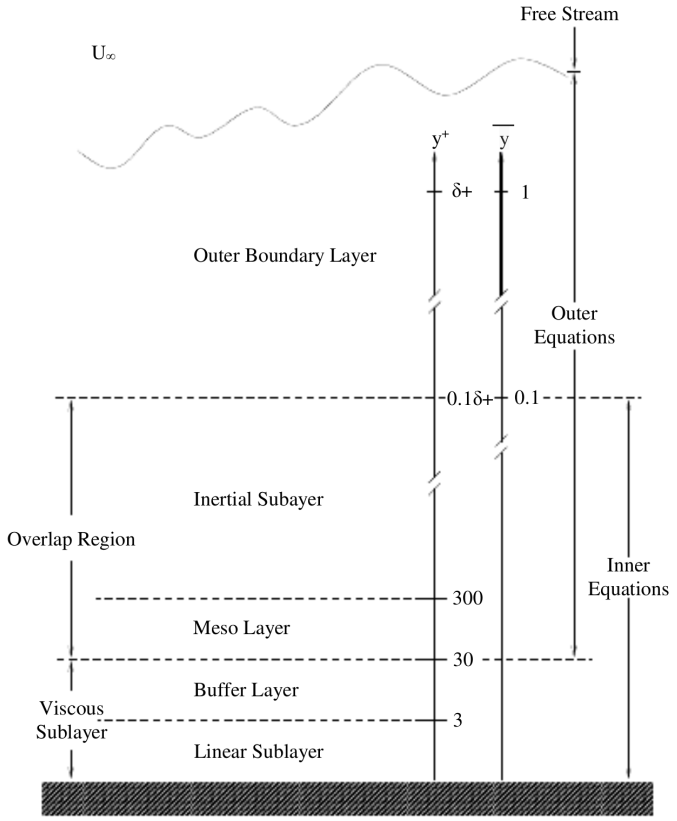
\includegraphics[scale=0.2]{Regionofturbulentboundarylayer}
 \caption{Regions of the turbulent boundary layer}
  \label{fig:fig14}
\end{figure}
From the figure(2.2) the inner layer consists of: the viscous linear sublayer($0<{y^+}<5$), the buffer sublayer($5<{y^+}<30$) and the inertial sublayer($30<{y^+}<200-300$) where ${y^+}$ is the normalised
distance tot he wall calculated as:
\begin{equation}
{y^+}={\frac{{{C_{\mu}}^{1/4}}{k^{1/2}}}{\nu}}y
\end{equation}
The molecular viscosity dominates the viscous sub-layer, and turbulence effects are minimal. The turbulent layer viscosity dominates the inertial sub-layer, making molecular viscosity irrelevant.
Both turbulence and molecular viscosity are equally relevant in the buffer layer. \\
\begin{figure}[H]
 \centering
 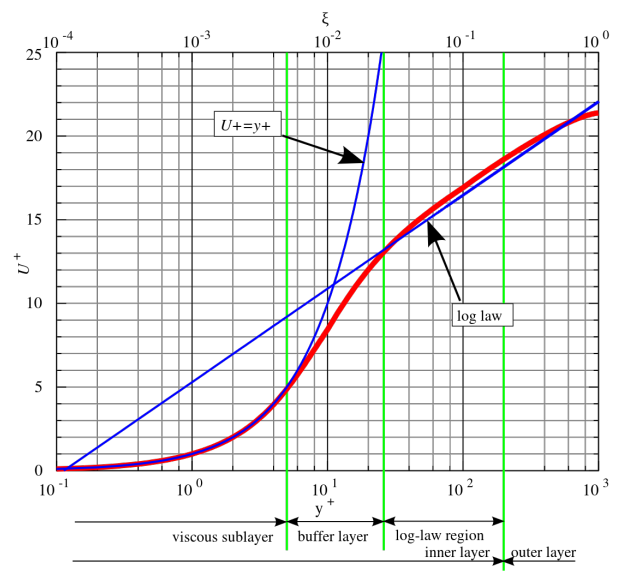
\includegraphics[scale=0.3]{Lawofthewall}
 \caption{Law of the wall}
  \label{fig:fig15}
\end{figure}
The assumptions described allow for the use of simple relations to represent the behavior of influencing variables in the near-wall region (as functions of wall distance).
Figure(2.3) depicts the relationship between dimensionless velocity U + and y +. (the red line represents the experimental observations and the two blue lines represent the two derived profiles).
The experimental results were best suited by the linear profile in the viscous sublayer and the logarithmic profile in the inertial sublayer, with the buffer sublayer serving as a smooth transition between the two.
As a result, the first cell center should be placed in either the viscous linear sublayer or the inertial sublayer. Because the buffer sublayer reflects a transition from linear to log, it should be avoided. 
Placing the first cell in the linear sublayer is assigned for low Reynolds turbulence modeling while placing in the inertial(log-layer) is a characteristic of high Reynolds turbulence modeling. In OpenFOAM
wall function for the field k is denoted with kqRWallFunction, for field $\omega$ omegaWallFunction and the correction ${\mu}_t$ is done in nutWallFunction.
\subsection{Automatic wall treatment for k-$\omega$ sst turbulence model}
The equation has a known solution in both the viscous and inertial (log-layer) sublayers, the k-$\omega$ sst turbulence model does not require extra damping functions to behave as a low Reynolds model.
Because the $\omega$ equation has a known solution in both viscous and inertial(log-layer) sublayer. Menter devised a blending technique based on this feature that enables a smooth shift from high to low Reynolds formulation and vice versa.
Despite the smooth shift, the buffer layer is not correctly represented by automatic wall treatment. 
\begin{equation}
{\omega}={\sqrt{{{{{\omega}^2}_{vis}}}+{{{{\omega}^2}_{log}}}}}
\end{equation}
where ${\omega}_{vis}$ and ${\omega}_{log}$ are defined as follows:
\begin{equation}
{{\omega}_{vis}}={\frac{6\mu}{{{\beta}_1}{\rho}{y^2}}}
\end{equation}
\begin{equation}
{{\omega}_{log}}={\frac{{k}^{1/2}}{\kappa {{C_{\mu}}^{1/4}} y}}
\end{equation}
The value of $\omega$ for the cell adjacent to the wall is obtained from eqaution(2.48). In these cells the production term G is given by:
\begin{equation}
G={G_{vis}}   (if {y^+}\le{{{y}^+}_{lam}})
\end{equation}
\begin{equation}
G={{G}_{log}} (if {{y^+}}\ge{{{y}^+}_{lam}})
\end{equation}
\begin{equation}
{G_{vis}}=0
\end{equation}
\begin{equation}
{G_{log}}={\frac{{{C}^{1/4}}_{\mu} {{k}^{1/2}}({{\mu}_t}+{\mu})\vert{{\triangledown \overline{u}}}\vert}{\kappa y {\rho}}}
\end{equation}
where
\begin{equation}
{{y^+}_{lam}}={\frac{{ln\bigg(max\bigg(E{{y^+}_{lam}},1\bigg)\bigg)}}{\kappa}}
\end{equation}
where E is a dimensional constant with default value of 9.8 and ${y}^+$ from equation(2.47) are calculated.
\chapter{Case setup}d Des
\section{A test case}
With the help of the OpenFOAM tutorial case study, a test case was set up. For the simulation of multiphase flow, the NACA0012 aerofoil geometry and blockMeshDict file are used 
from the compressible flow tutorial in OpenFOAM. The turbulence model adopted in this thesis is the k-$\omega$ sst model, used in the study tutorial. To set up the case for multiphase flow, 
another case study tutorial is used: multiphase/interFoam/RAS/propeller. For the multiphase simulation, the three folders are set using the case setup done in the 
study tutorial of propeller $\textit {0/, constant/, system/}$. The mass transfer model used in this tutorial is Schnerr-Sauer, which synchronizes with this thesis and 
also assists with setting up the 3 folders to run the simulation properly. In the working directory, copy the geometry from the study tutorial of compressible flow over 
the NACA0012 $\&$ folder setup from the tutorial of the propeller from multiphase. This case setup contains three folders $\textit {0/, constant/, and system/}$, and a slight modification 
is made to all three of them as outlined below.
\section{Computational domain}
The flow field around the hydrofoil is modeled in three-dimension with negligible dimension in span wise direction. 
\section{Boundary and initial condition}
The boundary condition and parameters of work condition  are taken from the reference  \cite{Zhao2021} which is stated below:\\
\begin{table}[h]
    \centering
    \begin{tabular}{|c|c|}
    \hline
        Hydrofoil & Wall \\
    \hline
        inlet & Velocity \\ 
    \hline
       Outlet & Pressure  \\
    \hline
       Top and Bottom & Symmetry \\
   \hline
    \end{tabular}
    \caption{Boundary condition}
    \label{tab:BC}
\end{table}\\





The parameter of working condition is stated below:
\begin{table}[h]
    \centering
    \begin{tabular}{|c|c|}
    \hline
        Velocity(U) & 5 m/s \\
    \hline
        Cavitation number ($\sigma$) & 0.8 \\ 
    \hline
     Turbulence kinetic energy(K) & 0.0185 \\
    \hline
    Specific dissipation rate($\omega$) & 621.626 \\
    \hline
    pressure($P_v$) & 9358.6848 N/${m}^2$\\
    \hline
    Reference pressure($P_{out}$) &  0.203e5 N/${m}^2$ \\
    \hline
    Chord length(C) & 100 mm \\
    \hline
    Angle of attack($\alpha$) & ${3.2}^{\circ}$ to ${8}^{\circ}$ \\
   \hline
    \end{tabular}
    \caption{parameters of work condition}
    \label{tab:PC}
\end{table}

\section{Case folder setup}
\subsection{$\textbf {0 Folder}$} This folder should be initilized with the working parameters such as velocity as $\textbf{\textit {U}}$ which is a reference velocity, $\textbf{\textit{p}}_{\textbf{\textit {\_rgh}}}$  reference pressure, $\textbf{\textit {omega}}$ specific dissipation rate, 
$\textbf{\textit {K}}$ turbulence kinetic energy, $\textbf{\textit {nut}}$, $\textbf{\textit {alpha.water}}$ vapour fraction respectively. Inorder to include the angle of attack on the hydrofoil it 
is better to specify the velocity as $V_x$=V$cos \alpha$ and $V_z$=$V sin \alpha$(normal direction is in z direction). The internalField and boundaryField of each files in the $0/$folder are stated below:\\ 
\begin{table}[h]
\centering
\begin{tabular}{|ll|ll|lll}
\cline{1-4}
\multicolumn{1}{|l|}{Parameters} & internalField & \multicolumn{2}{l|}{boundaryField}    &  &  &  \\ \cline{1-4}
\multicolumn{2}{|l|}{}    & \multicolumn{1}{l|}{freestream} & wall &  &  &  \\ \cline{1-4}
\multicolumn{1}{|l|}{U} & uniform $\$Uinlet$ & \multicolumn{1}{l|}{ type:            freestreamVelocity} &  type:            noSlip &  &  &  \\ \cline{1-4}
\multicolumn{1}{|l|}{pOut} & uniform $\$pOut$ & \multicolumn{1}{l|}{type:            freestreamPressure} &type:            fixedFluxPressure  &  &  &  \\ \cline{1-4}
\multicolumn{1}{|l|}{omegaInlet} & uniform $\$omegaInlet$ & \multicolumn{1}{l|}{type:            inletOutlet} & type:           omegaWallFunction &  &  &  \\ \cline{1-4}
\multicolumn{1}{|l|}{kInlet} & uniform $\$kInlet$ & \multicolumn{1}{l|}{type:           calculated} & type:            kqRWallFunction  &  &  &  \\ \cline{1-4}
\multicolumn{1}{|l|}{nut} & uniform 0  & \multicolumn{1}{l|}{type:            calculated} & type:            nutkWallFunction &  &  &  \\ \cline{1-4}
\end{tabular}
\caption{Condition of parameters of each files of 0$/$ folder}
 \label{tab:PC}
\end{table}
\begin{table}[h]
\centering
\begin{tabular}{|l|l|lll|}
\hline
Parameter& internalField  & \multicolumn{3}{l|}{boundaryField}                            \\ \hline
&  & \multicolumn{1}{l|}{inlet} & \multicolumn{1}{l|}{outlet} &  wall \\ \hline
alpha.water & uniform 1 & \multicolumn{1}{l|}{type:            fixedValue} & \multicolumn{1}{l|}{type:            inletOutlet} &type:            zeroGradient  \\ \hline
\end{tabular}
\caption{Condition of parameter of alpha.water files of 0$/$ folder}
\label{tab:PC}
\end{table}



In boundaryField, the freestream takes the value as uniform as declared in the internalField. The wall in the boundaryField is nothing but hydrofoil and some parameters requires 
value which is also declared from the internalField.

\subsection{Constant folder}
This folders enclosed with 4 files such as $\textit{g}/$, $\textit{momentum transport}/$, $\textit{phaseChangeProperties}/$, $\textit{transportProperties}/$. There are also two folders geometry 
and polyMesh. In $\textit{geometry}/$, the folder is enclosed with NACA0012.obj file which helps to run $\textit{ \$/blockMesh}$ command in the working directory to generate $\textit{polyMesh}/$ folder in the constant folder. This
folder carries files such as $\textit{boundary}/$, $\textit{face}/$, $\textit{neighbor}/$, $\textit{owner}/$, $\textit{points}/$.\\
The $\textit{momentumTransport/}$ file is the place for the declaration of turbulence model.
\begin{table}[h]
\centering
\begin{tabular}{|lll|}
\hline
\multicolumn{3}{|l|}{momentumTransport}                            \\ \hline
\multicolumn{1}{|l|}{simulationType } & \multicolumn{1}{l|}{RAS} & model:          kOmegaSST \\ \hline
\end{tabular}
\caption{Parameters in momentumTransport}
\label{tab:PC}
\end{table}
\begin{table}[h]
\centering
\begin{tabular}{|lll|}
\hline
\multicolumn{3}{|l|}{PhaseChangeProperties}                            \\ \hline
\multicolumn{1}{|l|}{phaseChangeModel} & \multicolumn{1}{l|}{SchnerrSauer} & SchnerrSauerCoeffs on \\ \hline
\multicolumn{1}{|l|}{pSat(saturation vapor pressure)} & \multicolumn{2}{l|}{9358.6848}    \\ \hline
\end{tabular}
\caption{Parameters in phaseChangeProperties}
\label{tab:PC}
\end{table}
The $\textit{phaseChangeProperties/}$ file is the place for the declaration of mass transfer model and saturation vapor pressure.
$/textit[transportProperties]/$ is the place to declare the phase of a mixture, its properties, as well as the cavitation number.
\begin{table}[h]
\centering
\begin{tabular}{|ll|}
\hline
\multicolumn{2}{|l|}{transportProperties}    \\ \hline
\multicolumn{1}{|l|}{phases} &water vapour  \\ \hline
\multicolumn{1}{|l|}{pSat} & 9358.6848 \\ \hline
\multicolumn{1}{|l|}{sigma(cavitation number) } & 0.8 \\ \hline
\end{tabular}
\caption{Parameters in transportProperties}
\label{tab:PC}
\end{table}
\subsection{System folder}
This folder contains files such as  $\textit{blockMeshDict}/$, $\textit{controlDict}/$, $\textit{decomposeParDict}/$, $\textit{extrudeMeshDict}/$, $\textit{fvScheme}/$, $\textit{fvSolution}/$.
\subsubsection{Time step control}
The court number affects the reliability and stability of the unstable flow simulation. The maxCo should be set around 5.Therefore a detlaT of 1e-5 seconds/system/controDict file. 
Note that cavitating flow calculations should always be initiated from a flow field. When cavitation is toggled on, simulation must be restarted from the current flow field.
\subsubsection{Discretisation schemes}
In OpenFOAM, the free surface treatment does not account for turbulence. All free surface simulations can be viewed as direct numerical simulations (DNS). 
Therefore there is a high requirement for the mesh resolution of the interface. The solver uses the multidimensional universal limiter for explicit solutions (MULES) to maintain the 
boundedness of the phase fraction, regardless of the underlying numerical scheme, mesh structure, etc. The choice of schemes for convection is therefore not restricted to those that 
are strongly stable or bounded, e.g. upwind differencing.
\subsubsection{Solution and algorithm control}



















































  
  
  
  
  
  
  
  
  
  
  
  
  
  
  
  
  
  
  
  
  
  
  
  
  
  
  
  
  
  
  
  
  
  
  
  
  
  
  
  
  
  
  
  
  
  
  
  
  
  
  
  
  
  
  
  
  
  
  
  
  
  
  
  
  
  
  
  
  
  
  
  
	        
 




















































 
